\documentclass{article}

%\usepackage[utf8]{inputenc}
\usepackage{graphicx}

\title{DB Modelling excercises}
\author{Claudia Vasallo}
\date{}
\begin{document}
\maketitle

\section{Excercise 1: Vueling}
\underline{Models} lists all plane models identified by a model id and stores its name, features and capacity. \underline{Planes} lists all planes the company owns identified by a plane id and relates to its model. \underline{Seats} identifies the seats of every plane by their seat number and plane id and stores their features.
\begin{figure}[h!]
 \centering
  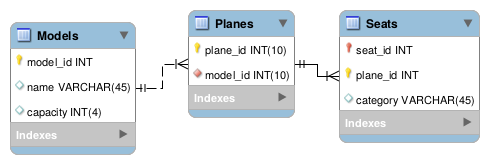
\includegraphics[width=0.8\linewidth]{vueling.png}
  \caption{Model for Vueling database}
  \label{fig:Vueling DB}
\end{figure}

\section{Excercise 2: Paintings}
\underline{Paintings} defines the paintings by a painting id, relates their author and stores their price, wheter or not it has been sold (Status) and in case it has been sold, the buye id. \underline{Buyers} defines the buyers with a buyer id and stores their names and DNI. 
\begin{figure}[h!]
 \centering
  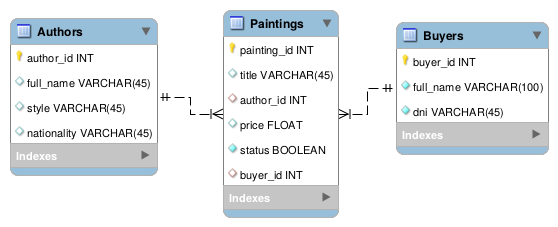
\includegraphics[width=0.8\linewidth]{paintings.png}
  \caption{Model for the Paintings Store database}
  \label{fig:Paintings Store DB}
\end{figure}


\section{Excercise 3: Stube}
\underline{User} defines the users with their user id and stores their usernames and passwords. \underline{Videos} stores the videos identified by its video id and the user id of the publisher and stores its title, description and url. 
\begin{figure}[h!]
 \centering
  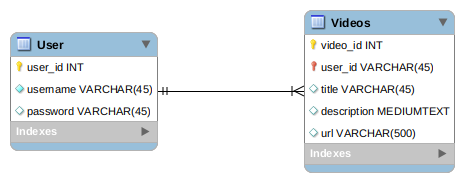
\includegraphics[width=0.8\linewidth]{stube.png}
  \caption{Model for the Stube database}
  \label{fig:Stube DB}
\end{figure}

\section{Excercise 5: Amazon Books}
\underline{Books} identifies each book by its book id and stores its title, author id, available stock and price. \underline{Authors} identifies an author by the authors by their author id and stores their full names and addresses. \underline{Users} identifies the users with a user id and stores their usernames, emails and passwords. \underline{Invoices} identifies a invoice by its invoice id and relates the user that produced the invoice.  \underline{Purchases} is a joining table that relates the invoices to the purchased items and quantities to be included in the invoice.
\begin{figure}[h!]
 \centering
  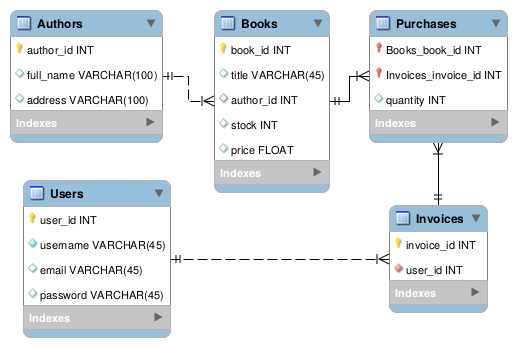
\includegraphics[width=0.8\linewidth]{amazon.png}
  \caption{Model for the Amazon Books database}
  \label{fig:Amazon Books DB}
\end{figure}

\section{Excercise 5: Social Network}
\underline{Users} identifies each user by its user id and stores its username, email and password. \underline{Photos} identifies each photo published by a photo id and its author's user id and stores its address and url where it is located. \underline{Friendship} is a joining table that relates two users that have become friends and stores their "How we met" story.
\begin{figure}[h!]
 \centering
  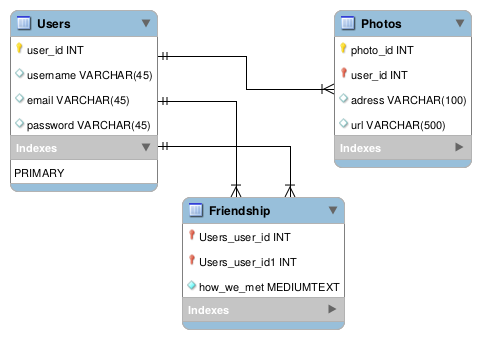
\includegraphics[width=0.8\linewidth]{xarxa.png}
  \caption{Model for the Social Network database}
  \label{fig:Social Network DB}
\end{figure}



\end{document}


